\section{Application}

\subsection{Perihelion precession of Mercury}

In this part we are going to apply the results that we have found to interpret the
perihelion precession of Mercury. In fact, in past hundred years, this problem
was never been explained correctly, until the appearance of the general relativity.
We start by looking for the analytic formulas and thanks to the numerical tools that we
have acquired, then we can move on to the numerical simulation to visualize the orbit of Mercury.

In Newton's classical case, most of the movements of the planet is described by the
Binet's formula:
%
\begin{equation}\label{Binet classique}
	\frac{\mathrm{d}^2u}{\mathrm{d}\phi^2}+u=\frac{GM}{h^2}
\end{equation}
%
with $u=1/r$ and $h$ the specific angular momentum with $\textbf{h}=\textbf{L}/m$.

The demonstration of the Binet's equation from the law of Newtonian movement is given in
the lecture of the course \textit{4P017 Gravitation} of the first semester. We quote the
link of the lecture here: (\url{http://syrte.obspm.fr/~souchay/cours2012/coursII.pdf}). The
complete demonstration begins from page 3.

The equation \eqref{Binet classique} can be integrated, with the demonstration in the
lecture we get:
\begin{equation}\label{orbit classique}
	u=\frac{1}{r}=\frac{GM}{h^2}\left[ 1+\sqrt{1+\frac{2h^2E}{G^2M^2m}}
	\mathrm{cos}\left( \theta-\theta_0\right)\right]
\end{equation}
%
with $E$ the total energy of the planet. We can also write it in this form:
%
\begin{equation}
	r=\frac{1}{u}=\frac{p}{1+e\mathrm{cos}\left( \theta-\theta_0\right) }
\end{equation}
%
with $p=\frac{h^2}{GM}$ and the eccentricity $e=\sqrt{1+\frac{2h^2E}{G^2M^2m}}$.
If $0<e<1$, the orbit is an stable ellipse.

In the case of relativity, the Binet's equation is consisted of the classical Binet's
equation and a term of relativistic correction. This formula which can be demonstrated from
the Schwarzchild metric given by: 
%
\begin{equation}
	\frac{\mathrm{d}^2u}{\mathrm{d}\phi^2}+u=\frac{GM}{h^2}+\frac{3GM}{c^2}u^2
\end{equation}
%
The ratio between the corrective term $3GMu^2$ and the classical term $\frac{GM}{h^2}$ gives $3v^2$
and as the average orbital velocity of Mercury in units of $c$\footnote{In S.I., we have $v = 47.36 \, \mathrm{km}.\mathrm{s}^{-1}$.} is of magnitude $10^{-4}$ it is negligible and we can
treat it in perturbation in first approximation. We substitute the solution
into the corrective term :
%
\begin{equation}
	\frac{\mathrm{d}^2u}{\mathrm{d}\phi^2}+u=\frac{GM}{h^2}+\frac{3GM}{c^2}
	\left[\frac{GM}{h^2}\left(1+e\mathrm{cos} \left( \theta-\theta_0\right)\right)
	\right] ^2
	\approx \frac{GM}{h^2}+\frac{3G^3M^3}{c^2h^4}+6\frac{G^3M^3}{c^2h^4}e\mathrm{cos}
	\left( \theta-\theta_0\right)
\end{equation}
%
The second term can be neglected because it's a very tiny correction before the first term.
So we have:
\begin{equation}
	\frac{\mathrm{d}^2u}{\mathrm{d}\phi^2}+u=\frac{GM}{h^2}+6\frac{G^3M^3}{c^2h^4}e
	\cos \left( \theta-\theta_0\right)
\end{equation}
%
We let:
%
\begin{equation}
\begin{aligned}
	\frac{\mathrm{d}^2u_1}{\mathrm{d}\phi^2}+u_1=\frac{GM}{h^2}
	\\
	\frac{\mathrm{d}^2u_2}{\mathrm{d}\phi^2}+u_2=6\frac{G^3M^3}{c^2h^4}e\cos
	\left( \theta-\theta_0\right)
\end{aligned}
\end{equation}

$u_1$ is the same with \eqref{orbit classique}, and $u_2$ has a particular solution:
%
\begin{equation}
	u_2=3\frac{G^3M^3}{c^2h^4}e\left( \theta-\theta_0\right)\sin
	\left( \theta-\theta_0\right)
\end{equation}
%
We get:
%
\begin{equation}
\begin{aligned}
	u=u_1+u_2=\frac{GM}{h^2}\left(1+e\mathrm{cos} \left( \theta-\theta_0\right)
	+3\frac{G^2M^2}{c^2h^2}e\left( \theta-\theta_0\right)\mathrm{sin}
	\left( \theta-\theta_0\right)\right)
	\\
	\approx \frac{GM}{h^2}\left( 1+e\mathrm{cos}\left( 1-3\frac{G^2M^2}{c^2h^2}\right)
	\left( \theta-\theta_0\right)\right) 
\end{aligned}
\end{equation}
%
Comparing to the Newton's stable orbit, we see that a precession appears:
%
\begin{equation}
	\left( 1-3\frac{G^2M^2}{c^2h^2}\right) \left( \theta-\theta_0\right)=2n\pi,
	\qquad n=1,2,3...
\end{equation}
%
We have:
%
\begin{equation}
	\phi=\left( \theta-\theta_0\right)=\frac{2n\pi}{1-3\frac{G^2M^2}{c^2h^2}}\approx
	2n\pi \left( 1+3\frac{G^2M^2}{c^2h^2}\right) ^2
\end{equation}
%
And finally:
%
\begin{equation}
	\Delta\phi=6\pi\frac{G^2M^2}{c^2h^2} 
\end{equation}
%
With numerical application, we see the precession of the Mercury is about $43''$ per
century, which accords with the observations.

\subsection{Numerical simulation of the Mercury's orbit}

In this part we are going to write programs to simulate the orbit of the perihelion
precession of Mercury by using the numerical methods. In fact solving the problem between
analytic method and numerical method is radically different. Although to solve some
equations analytically is very difficult even impossible, to solve it with numerical
method is quite easy. In our case, the classical Newtonian Binet's equation can be
solved analytically, but Binet's equation with relativistic correction is very
difficult to solve. We try to resolve this equation numerically in order to plot the
revolution's orbit of Mercury. Moreover, because of the non-linearity of Einstein field
equations, to solve it in general cases is impossible. So the numerical method becomes
essential in this research area. Today, there is a research branch called numerical
relativity concentrating on the numerical methods and algorithms to solve the problem.

To solve the differential equation, we have tried different numerical methods like the
Euler method, the Runge–Kutta methods, etc. Euler method is the simplest method but
missing enough precision. The fourth order Runge–Kutta methods(RK4) is widely used in the
numerical calculation. In our case, we chose the Runge–Kutta methods for the
simulation.

For the programming language, we have written in C language and Fortran. We quote some
essential codes:
\\
\\
RK4 in C
\begin{lstlisting}[language=C,basicstyle=\small\ttfamily]
void rk4(int p, real* u_i, real t_i, real h, real* (*ptr_f)
(real, real*, int), real* u_i_plus){
int j = 0;
real* k1 = NULL;real* k2 = NULL;real* k3 = NULL;real* k4 = NULL;
real* stock = NULL;
stock = (real*)calloc((size_t)p, sizeof(real));
if(stock == NULL){
	fprintf(stderr, "Erreur d'allocation !\n");
	exit(EXIT_FAILURE);}
k1 = (*ptr_f)(t_i, u_i, p);
for(j=0;j<p;j++){stock[j] = u_i[j] + k1[j]*h/2;}
k2 = (*ptr_f)(t_i + h/2, stock, p);
for(j=0;j<p;j++){stock[j] = u_i[j] + k2[j]*h/2;}
k3 = (*ptr_f)(t_i + h/2, stock, p);
for(j=0;j<p;j++){stock[j] = u_i[j] + k3[j]*h;}
k4 = (*ptr_f)(t_i + h, stock, p);
for(j=0;j<p;j++){u_i_plus[j] = u_i[j] + (k1[j] 
+ 2*(k2[j] + k3[j]) + k4[j])*h/6;}
\end{lstlisting}
RK4 in Fortran (program given by P. Depondt in the course \textit{Physique numérique})
\begin{lstlisting}[language=Fortran,basicstyle=\small\ttfamily]
subroutine rk4(x,y,dx,n,deriv)
implicit none
integer           , intent(in)    :: n
real              , intent(in)    :: x, dx
real, dimension(n), intent(inout) :: y
real                              :: ddx
real, dimension(n)                :: yp, k1, k2, k3, k4
ddx = 0.5*dx
call deriv(x,y,k1,n)      ; yp=y+ddx*k1
call deriv(x+ddx,yp,k2,n) ; yp=y+ddx*k2
call deriv(x+ddx,yp,k3,n) ; yp=y+dx*k3
call deriv(x+dx,yp,k4,n)  ; y =y+dx*(k1+2.0*k2+2.0*k3+k4)/6.0
end subroutine rk4
\end{lstlisting} 

The program for calculating the orbit in C:
\begin{lstlisting}[language=C,basicstyle=\small\ttfamily]
/* Fonction qui definie le second membre */
real* newton(real t, real* u, int p){
	real* second_membre = NULL;
	second_membre = (real*)calloc((size_t)p, sizeof(real));
	if(second_membre == NULL){
		fprintf(stderr, "Erreur d'allocation !\n");
		exit(EXIT_FAILURE);}
	second_membre[0] = u[2];
	second_membre[1] = u[3];
	second_membre[2] =   u[0]*u[3]*u[3] - k/u[0]/u[0]
	                   - c/u[0]/u[0]/u[0]/u[0];
	second_membre[3] = -2*u[2]*u[3]/u[0];
	return second_membre;}
\end{lstlisting}

Here we try to solve Binet's equation (classical and relativistic). Binet's equation is a second order equation. We can transform it in two first order equations. We create two arrays to stock the values of $r\left(t \right) $ and $r'\left( t\right) $. We can export all these values in a file. Here is the program for calculating the orbit in Fortran:
\begin{lstlisting}[language=Fortran,basicstyle=\small\ttfamily]
subroutine derivenewton(phi,r,d,n)
implicit none
integer, intent(in) :: n
real, intent(in) :: phi
real, dimension(n), intent(in) :: r
real, dimension(n), intent(out) :: d
d(1) = r(2)
d(2) = G*M/L**2-u(1)
end subroutine derivenewton

subroutine deriverelat(phi,r,d,n)
d(1) = r(2)
d(2) = G*M/L**2-u(1)+3*G*M*u(1)**2
end subroutine deriverelat
\end{lstlisting}

Then we can plot the $r(\phi)$ or $r(t)$ stocked in the file by using Gnuplot or Scilab.

In fact the precession of the Mercury is so slow that we can not visualize clearly the difference. So we have changed the parameters in order to obtain a better graph which present the essence of the movement.


\begin{figure}
	\begin{center}
		\subfloat[Classic trajectory]{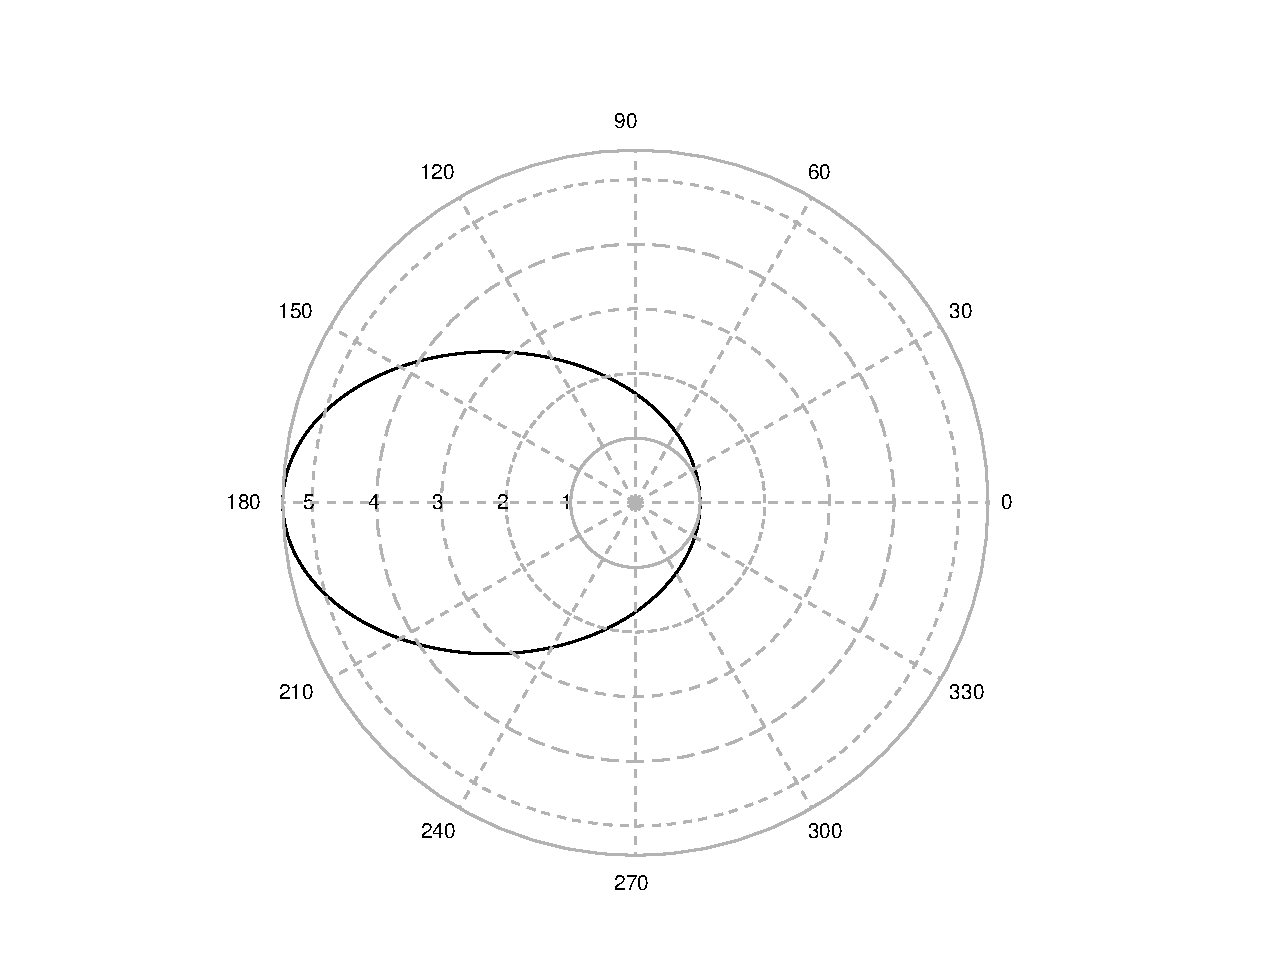
\includegraphics[scale=0.3]{ellipse.pdf}
		\label{flottants:precession:classique}}
		\subfloat[Corrected trajectory]{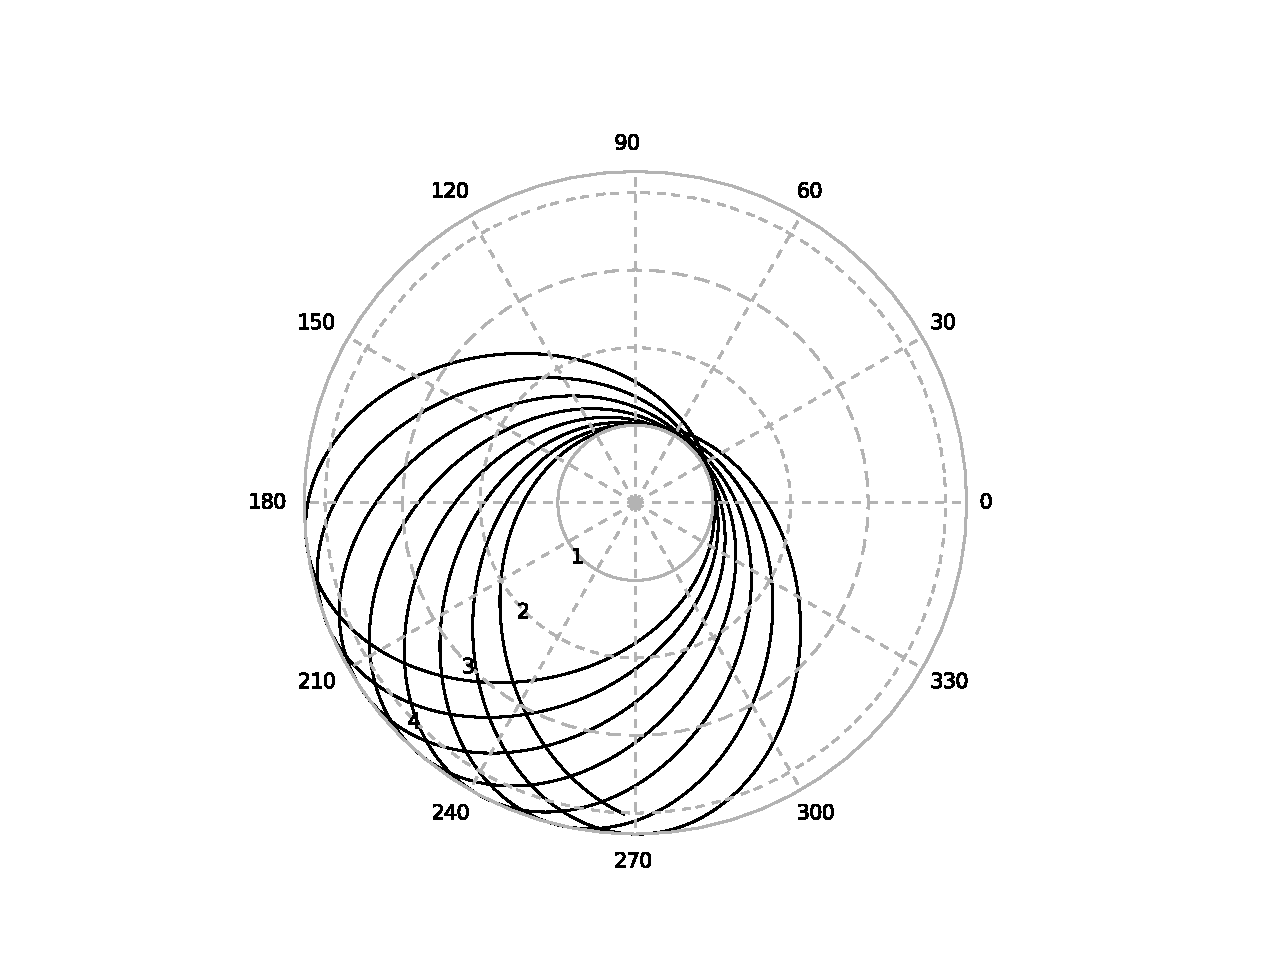
\includegraphics[scale=0.3]{precession.pdf}
		\label{flottants:precession:precession}}
	\end{center}
	\caption{We can see on these figures the differences between classic and corrected
	         trajectory. The first is a simple ellipse while the latter is an ellipse which
			 precess with time.}
	\label{flottants:precession:differences}
\end{figure}

\section{Conclusion}

In this project, we have seen how general relativity works and more particularly, we can
easily come back to the Newtonian theory by using some approximations or by removing simply
a part of a calculus. From this narrow link between these two theories, we also understood
that we could obtain better results by using the general relativity for problems than by
using gravitation.
Indeed, the fact that the empiric force defined by Newton centuries ago can be corrected by
a factor, allows us to apply the general relativity to some problems that Newtonian theory
could not resolve.
In our project, we have studied the perihelion precession of Mercury that can be only
understood by using general relativity, as the Newtonian theory predicts an invariable
ellipse.
However, this experiment is not the only one. There are many experimental justifications
confirming general relativity. For example, the redshift or the curvature of light rays.
And every time this approach passes the experimental test.

At the beginning of the project, we have planned to look for others solutions to Einstein
field equations. It might be also interesting to study another experiment to test the
general relativity or to compare the results that we have obtained by using another metric
of Einstein field equations like the Kerr metric. However, as the Schwarzchild metric has
already such a lot of interesting things, in the second part of our study, we changed to
looking for the application and the numerical simulation of the Schwarzchild metric, like
the perihelion precession of Mercury, in order to understand more clearly the correction
of Schwarzchild to Newton’s law. 